\documentclass[
  man,
  floatsintext,
  longtable,
  nolmodern,
  notxfonts,
  notimes,
  colorlinks=true,linkcolor=blue,citecolor=blue,urlcolor=blue]{apa7}

\usepackage{amsmath}
\usepackage{amssymb}



\usepackage[bidi=default]{babel}
\babelprovide[main,import]{english}


% get rid of language-specific shorthands (see #6817):
\let\LanguageShortHands\languageshorthands
\def\languageshorthands#1{}

\RequirePackage{longtable}
\RequirePackage{threeparttablex}

\makeatletter
\renewcommand{\paragraph}{\@startsection{paragraph}{4}{\parindent}%
	{0\baselineskip \@plus 0.2ex \@minus 0.2ex}%
	{-.5em}%
	{\normalfont\normalsize\bfseries\typesectitle}}

\renewcommand{\subparagraph}[1]{\@startsection{subparagraph}{5}{0.5em}%
	{0\baselineskip \@plus 0.2ex \@minus 0.2ex}%
	{-\z@\relax}%
	{\normalfont\normalsize\bfseries\itshape\hspace{\parindent}{#1}\textit{\addperi}}{\relax}}
\makeatother




\usepackage{longtable, booktabs, multirow, multicol, colortbl, hhline, caption, array, float, xpatch}
\setcounter{topnumber}{2}
\setcounter{bottomnumber}{2}
\setcounter{totalnumber}{4}
\renewcommand{\topfraction}{0.85}
\renewcommand{\bottomfraction}{0.85}
\renewcommand{\textfraction}{0.15}
\renewcommand{\floatpagefraction}{0.7}

\usepackage{tcolorbox}
\tcbuselibrary{listings,theorems, breakable, skins}
\usepackage{fontawesome5}

\definecolor{quarto-callout-color}{HTML}{909090}
\definecolor{quarto-callout-note-color}{HTML}{0758E5}
\definecolor{quarto-callout-important-color}{HTML}{CC1914}
\definecolor{quarto-callout-warning-color}{HTML}{EB9113}
\definecolor{quarto-callout-tip-color}{HTML}{00A047}
\definecolor{quarto-callout-caution-color}{HTML}{FC5300}
\definecolor{quarto-callout-color-frame}{HTML}{ACACAC}
\definecolor{quarto-callout-note-color-frame}{HTML}{4582EC}
\definecolor{quarto-callout-important-color-frame}{HTML}{D9534F}
\definecolor{quarto-callout-warning-color-frame}{HTML}{F0AD4E}
\definecolor{quarto-callout-tip-color-frame}{HTML}{02B875}
\definecolor{quarto-callout-caution-color-frame}{HTML}{FD7E14}

%\newlength\Oldarrayrulewidth
%\newlength\Oldtabcolsep


\usepackage{hyperref}




\providecommand{\tightlist}{%
  \setlength{\itemsep}{0pt}\setlength{\parskip}{0pt}}
\usepackage{longtable,booktabs,array}
\usepackage{calc} % for calculating minipage widths
% Correct order of tables after \paragraph or \subparagraph
\usepackage{etoolbox}
\makeatletter
\patchcmd\longtable{\par}{\if@noskipsec\mbox{}\fi\par}{}{}
\makeatother
% Allow footnotes in longtable head/foot
\IfFileExists{footnotehyper.sty}{\usepackage{footnotehyper}}{\usepackage{footnote}}
\makesavenoteenv{longtable}

\usepackage{graphicx}
\makeatletter
\def\maxwidth{\ifdim\Gin@nat@width>\linewidth\linewidth\else\Gin@nat@width\fi}
\def\maxheight{\ifdim\Gin@nat@height>\textheight\textheight\else\Gin@nat@height\fi}
\makeatother
% Scale images if necessary, so that they will not overflow the page
% margins by default, and it is still possible to overwrite the defaults
% using explicit options in \includegraphics[width, height, ...]{}
\setkeys{Gin}{width=\maxwidth,height=\maxheight,keepaspectratio}
% Set default figure placement to htbp
\makeatletter
\def\fps@figure{htbp}
\makeatother







\usepackage{newtx}

\defaultfontfeatures{Scale=MatchLowercase}
\defaultfontfeatures[\rmfamily]{Ligatures=TeX,Scale=1}





\title{Level 1 Data Visualization: Plot the mtcars Dataset}


\shorttitle{Data Visualization Mini-project}


\usepackage{etoolbox}






\author{Lisa Zhu}



\affiliation{
{MA Program in the Social Sciences, University of Chicago}}




\leftheader{Zhu}

\date{2025-02-21}


\abstract{This document analyzes the mcar dataset, and presents the
relationship between several variables to demonstrate my ability using
ggplot.}

\keywords{ggplot2, data visualization}

\authornote{ 

\par{     The author is grateful to Dr.~Dowling and Mian Li for teaching
me how to use R and rendering a manuscript from
R.  Author roles were classified using the Contributor Role Taxonomy (CRediT; https://credit.niso.org/) as follows: Lisa
Zhu:   writing, designs}
\par{Correspondence concerning this article should be addressed to Lisa
Zhu, MA Program in the Social Sciences, University of Chicago, 1155 E
60th St., Chicago, IL 60615, USA, Email: lisazhu@uchicago.edu}
}

\makeatletter
\let\endoldlt\endlongtable
\def\endlongtable{
\hline
\endoldlt
}
\makeatother

\urlstyle{same}



\usepackage{booktabs}
\usepackage{longtable}
\usepackage{array}
\usepackage{multirow}
\usepackage{wrapfig}
\usepackage{float}
\usepackage{colortbl}
\usepackage{pdflscape}
\usepackage{tabu}
\usepackage{threeparttable}
\usepackage{threeparttablex}
\usepackage[normalem]{ulem}
\usepackage{makecell}
\usepackage{xcolor}
\usepackage{fontspec}
\usepackage{multicol}
\usepackage{hhline}
\newlength\Oldarrayrulewidth
\newlength\Oldtabcolsep
\usepackage{hyperref}
\makeatletter
\@ifpackageloaded{caption}{}{\usepackage{caption}}
\AtBeginDocument{%
\ifdefined\contentsname
  \renewcommand*\contentsname{Table of contents}
\else
  \newcommand\contentsname{Table of contents}
\fi
\ifdefined\listfigurename
  \renewcommand*\listfigurename{List of Figures}
\else
  \newcommand\listfigurename{List of Figures}
\fi
\ifdefined\listtablename
  \renewcommand*\listtablename{List of Tables}
\else
  \newcommand\listtablename{List of Tables}
\fi
\ifdefined\figurename
  \renewcommand*\figurename{Figure}
\else
  \newcommand\figurename{Figure}
\fi
\ifdefined\tablename
  \renewcommand*\tablename{Table}
\else
  \newcommand\tablename{Table}
\fi
}
\@ifpackageloaded{float}{}{\usepackage{float}}
\floatstyle{ruled}
\@ifundefined{c@chapter}{\newfloat{codelisting}{h}{lop}}{\newfloat{codelisting}{h}{lop}[chapter]}
\floatname{codelisting}{Listing}
\newcommand*\listoflistings{\listof{codelisting}{List of Listings}}
\makeatother
\makeatletter
\makeatother
\makeatletter
\@ifpackageloaded{caption}{}{\usepackage{caption}}
\@ifpackageloaded{subcaption}{}{\usepackage{subcaption}}
\makeatother

% From https://tex.stackexchange.com/a/645996/211326
%%% apa7 doesn't want to add appendix section titles in the toc
%%% let's make it do it
\makeatletter
\xpatchcmd{\appendix}
  {\par}
  {\addcontentsline{toc}{section}{\@currentlabelname}\par}
  {}{}
\makeatother

%% Disable longtable counter
%% https://tex.stackexchange.com/a/248395/211326

\usepackage{etoolbox}

\makeatletter
\patchcmd{\LT@caption}
  {\bgroup}
  {\bgroup\global\LTpatch@captiontrue}
  {}{}
\patchcmd{\longtable}
  {\par}
  {\par\global\LTpatch@captionfalse}
  {}{}
\apptocmd{\endlongtable}
  {\ifLTpatch@caption\else\addtocounter{table}{-1}\fi}
  {}{}
\newif\ifLTpatch@caption
\makeatother

\begin{document}

\maketitle


\setcounter{secnumdepth}{-\maxdimen} % remove section numbering

\setlength\LTleft{0pt}


\section{Objective}\label{objective}

The objective of this assignment is to practice constructing simple
visualizations using the \texttt{ggplot2} package in R. In this Level 1
assignment, you will work with simple datasets and focus on the most
commonly used layers and aesthetics. Most tasks are outlined in the
assignment script. You may want to review the
\href{../00_viz-walkthrough}{Data Visualization Walkthrough} before you
begin.

You may additionally or alternatively complete the
\href{../02_viz-level-2}{Level 2 Data Visualization assignment}. In
Level 2, you will work with a more complex dataset and perform
additional visualization tasks with less direct instruction. The Level 2
assignment has more opportunities to demonstrating meeting course
standards than this Level 1 assignment and is recommended for those who
are already comfortable with the tasks in this assignment. In
particular, the Level 2 assignment requires you to parse and use the
\texttt{theme()} layer in complicated ways to customize the appearance
of your plots.

\section{Instructions}\label{instructions}

\begin{enumerate}
\def\labelenumi{\arabic{enumi}.}
\tightlist
\item
  If you have not already done so, pull the latest changes from the
  \texttt{d2mr-assessment} repository to ensure you have the most
  up-to-date version of the assignment files. Confirm you are working in
  your clone of the repository.
\item
  Open \texttt{viz-level-1.qmd} in RStudio (you are here) and follow the
  instructions in the Setup section below to load and inspect the
  built-in \texttt{mtcars} dataset.

  \begin{itemize}
  \tightlist
  \item
    \textbf{Note:} You will perform simple data transformation in a
    chunk below to prepare the \texttt{mtcars} dataset for
    visualization. Save your transformed dataset to a new object,
    \texttt{mtcars.viz}, so you can still access the original dataset if
    needed.
  \end{itemize}
\item
  In the chunks provided, recreate each of the 6 plots (provided as .png
  files). You may need to render this notebook to see the images, or you
  can open the files directly. Recreate the plots as closely as
  possible, noting where you get stuck or have questions.

  \begin{itemize}
  \tightlist
  \item
    \textbf{Note:} The image files are included in the assessment repo
    in the \texttt{03\_data-viz/01\_viz-level-1/plots/} folder. If you
    don't see the files, you may have something in your .gitignore
    preventing them from being pulled. You can either edit your
    .gitignore to allow the files to be pulled or download the files
    directly from the GitHub repository.
  \end{itemize}
\item
  At several points in this document you will come across questions or
  non-coding exercises. Answer these questions in the text of this .qmd
  document, immediately below the question.
\item
  \emph{Optional:} Create additional plots using the \texttt{mtcars.viz}
  dataset or extend one or more of the plots above. Add your code to the
  ``Optional plotting'' section at the end of the document. Do not add
  this optional work to the main code chunks that recreate the plot
  images.
\end{enumerate}

\subsection{Setup}\label{setup}

I imported five packages: \textbf{tidyverse}, \textbf{knitr},
\textbf{janitor}, \textbf{quarto}, and \textbf{viridis}. I tried
installing \emph{apaquarto}, but didn't succeed using option 2. However,
I tried moving the extension folder from other directories to this one,
and it seems to be working.

\subsubsection{\texorpdfstring{Inspect the \texttt{mtcars}
dataset:}{Inspect the mtcars dataset:}}\label{inspect-the-mtcars-dataset}

Check the dataset: \texttt{?mtcars} \footnote{The data was extracted
  from the 1974 Motor Trend US magazine, and comprises fuel consumption
  and 10 aspects of automobile design and performance for 32 automobiles
  (1973--74 models).}.

The names of the variables in the \texttt{mtcars} dataset may not be
immediately clear. You can find a description of the variables in the
\texttt{mtcars} dataset by running \texttt{?mtcars} in the R console.

Consider the structure of the dataset, particularly the datatypes of
each variable. Based on the descriptions of each variable in the
documentation, not all variables are in the most appropriate format for
analysis or visualization.

QUESTIONS:

\begin{enumerate}
\def\labelenumi{\arabic{enumi}.}
\tightlist
\item
  Which variables in the \texttt{mtcars} dataset should be treated as
  numeric variables?
\end{enumerate}

mpg; cyl; disp; hp; wt; qsec; gear; carb; vs; am

\begin{enumerate}
\def\labelenumi{\arabic{enumi}.}
\setcounter{enumi}{1}
\tightlist
\item
  Of those you believe should be considered numeric, are they all also
  \emph{continuous} variables? Are there any \emph{non-continuous}
  numeric variables?
\end{enumerate}

\subsubsection{Continuous \& Categorical
Variables}\label{continuous-categorical-variables}

\begin{enumerate}
\def\labelenumi{\arabic{enumi}.}
\tightlist
\item
  continuous:
\end{enumerate}

\begin{itemize}
\tightlist
\item
  mpg
\item
  cyl
\item
  disp
\item
  hp
\item
  wt
\item
  qsec
\item
  gear
\item
  carb
\end{itemize}

\begin{enumerate}
\def\labelenumi{\arabic{enumi}.}
\setcounter{enumi}{1}
\tightlist
\item
  categorical:
\end{enumerate}

\begin{itemize}
\tightlist
\item
  vs
\item
  am
\end{itemize}

\begin{enumerate}
\def\labelenumi{\arabic{enumi}.}
\setcounter{enumi}{2}
\tightlist
\item
  Which variables in the \texttt{mtcars} dataset should be treated as
  factor variables?
\end{enumerate}

vs; am

\begin{enumerate}
\def\labelenumi{\arabic{enumi}.}
\setcounter{enumi}{3}
\tightlist
\item
  Of those you believe should be considered factors, are they ordered or
  unordered?
\end{enumerate}

Both are unordered.

\subsection{Data preparation}\label{data-preparation}

Based on your inspection of the \texttt{mtcars} dataset and your answers
to the above questions, use \texttt{dplyr}, \texttt{tidyr}, and
\texttt{forcats} functions to prepare the dataset for visualization.

You will need to change the data types for some variables. You may also
want to rename variables and factor levels for clarity. Renaming
variables and levels now can make your visualization simpler later, but
you can do it directly in the your plotting functions, too.

\subsection{Some Descriptive Data
Analysis}\label{some-descriptive-data-analysis}

\subsubsection{Miles per gallon (Objective 17; numeric
variable)}\label{miles-per-gallon-objective-17-numeric-variable}

Table~\ref{tbl-mean-median-sd-of-mpg-for-each-cylinder-type} shows the
mean, median, \& sd of miles per gallon for each cylinder type.

\begin{table}

{\caption{{mean, median, \& sd of miles per gallon for each cylinder
type}{\label{tbl-mean-median-sd-of-mpg-for-each-cylinder-type}}}
\vspace{-20pt}}

\global\setlength{\Oldarrayrulewidth}{\arrayrulewidth}

\global\setlength{\Oldtabcolsep}{\tabcolsep}

\setlength{\tabcolsep}{2pt}

\renewcommand*{\arraystretch}{1.5}



\providecommand{\ascline}[3]{\noalign{\global\arrayrulewidth #1}\arrayrulecolor[HTML]{#2}\cline{#3}}

\begin{longtable*}[c]{|p{0.75in}|p{0.75in}|p{0.75in}}



\ascline{0.75pt}{000000}{1-3}

\multicolumn{1}{>{\centering}m{\dimexpr 0.75in+0\tabcolsep}}{\textcolor[HTML]{000000}{\fontsize{11}{22}\selectfont{\global\setmainfont{Times New Roman}{cylinders}}}} & \multicolumn{1}{>{\centering}m{\dimexpr 0.75in+0\tabcolsep}}{\textcolor[HTML]{000000}{\fontsize{11}{22}\selectfont{\global\setmainfont{Times New Roman}{mean\_mpg}}}} & \multicolumn{1}{>{\centering}m{\dimexpr 0.75in+0\tabcolsep}}{\textcolor[HTML]{000000}{\fontsize{11}{22}\selectfont{\global\setmainfont{Times New Roman}{sd\_mpg}}}} \\

\ascline{0.75pt}{000000}{1-3}\endfirsthead 

\ascline{0.75pt}{000000}{1-3}

\multicolumn{1}{>{\centering}m{\dimexpr 0.75in+0\tabcolsep}}{\textcolor[HTML]{000000}{\fontsize{11}{22}\selectfont{\global\setmainfont{Times New Roman}{cylinders}}}} & \multicolumn{1}{>{\centering}m{\dimexpr 0.75in+0\tabcolsep}}{\textcolor[HTML]{000000}{\fontsize{11}{22}\selectfont{\global\setmainfont{Times New Roman}{mean\_mpg}}}} & \multicolumn{1}{>{\centering}m{\dimexpr 0.75in+0\tabcolsep}}{\textcolor[HTML]{000000}{\fontsize{11}{22}\selectfont{\global\setmainfont{Times New Roman}{sd\_mpg}}}} \\

\ascline{0.75pt}{000000}{1-3}\endhead



\multicolumn{1}{>{\centering}m{\dimexpr 0.75in+0\tabcolsep}}{\textcolor[HTML]{000000}{\fontsize{11}{22}\selectfont{\global\setmainfont{Times New Roman}{4.00}}}} & \multicolumn{1}{>{\centering}m{\dimexpr 0.75in+0\tabcolsep}}{\textcolor[HTML]{000000}{\fontsize{11}{22}\selectfont{\global\setmainfont{Times New Roman}{26.66}}}} & \multicolumn{1}{>{\centering}m{\dimexpr 0.75in+0\tabcolsep}}{\textcolor[HTML]{000000}{\fontsize{11}{22}\selectfont{\global\setmainfont{Times New Roman}{4.51}}}} \\





\multicolumn{1}{>{\centering}m{\dimexpr 0.75in+0\tabcolsep}}{\textcolor[HTML]{000000}{\fontsize{11}{22}\selectfont{\global\setmainfont{Times New Roman}{6.00}}}} & \multicolumn{1}{>{\centering}m{\dimexpr 0.75in+0\tabcolsep}}{\textcolor[HTML]{000000}{\fontsize{11}{22}\selectfont{\global\setmainfont{Times New Roman}{19.74}}}} & \multicolumn{1}{>{\centering}m{\dimexpr 0.75in+0\tabcolsep}}{\textcolor[HTML]{000000}{\fontsize{11}{22}\selectfont{\global\setmainfont{Times New Roman}{1.45}}}} \\





\multicolumn{1}{>{\centering}m{\dimexpr 0.75in+0\tabcolsep}}{\textcolor[HTML]{000000}{\fontsize{11}{22}\selectfont{\global\setmainfont{Times New Roman}{8.00}}}} & \multicolumn{1}{>{\centering}m{\dimexpr 0.75in+0\tabcolsep}}{\textcolor[HTML]{000000}{\fontsize{11}{22}\selectfont{\global\setmainfont{Times New Roman}{15.10}}}} & \multicolumn{1}{>{\centering}m{\dimexpr 0.75in+0\tabcolsep}}{\textcolor[HTML]{000000}{\fontsize{11}{22}\selectfont{\global\setmainfont{Times New Roman}{2.56}}}} \\

\ascline{0.75pt}{000000}{1-3}



\end{longtable*}



\arrayrulecolor[HTML]{000000}

\global\setlength{\arrayrulewidth}{\Oldarrayrulewidth}

\global\setlength{\tabcolsep}{\Oldtabcolsep}

\renewcommand*{\arraystretch}{1}

\end{table}

Figure~\ref{fig-mean-median-sd-of-mpg-for-each-cylinder-type} visualizes
the table above.

\begin{figure}

\caption{\label{fig-mean-median-sd-of-mpg-for-each-cylinder-type}mean,
median, \& sd of miles per gallon for each cylinder type}

\centering{

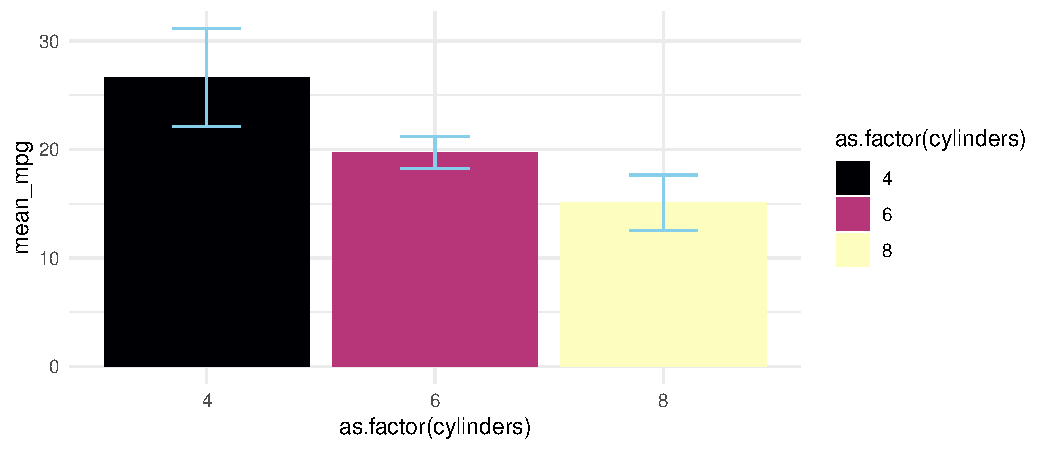
\includegraphics{data-visualization_files/figure-pdf/fig-mean-median-sd-of-mpg-for-each-cylinder-type-1.pdf}

}

\end{figure}%

\subsubsection{Engine (Obejctive 17; factor
variable)}\label{engine-obejctive-17-factor-variable}

Table~\ref{tbl-frequency-and-proportion-of-engine-being-v-shape-or-straight}
shows the frequency and proportion of engine by type.

\begin{table}

{\caption{{Summary Statistics for
Engine}{\label{tbl-frequency-and-proportion-of-engine-being-v-shape-or-straight}}}
\vspace{-20pt}}

\begin{longtable*}[t]{cc>{}c}
\\
\toprule
Engine & Count & Percentage\\
\midrule
0 & 18 & \cellcolor[HTML]{FDE725}{\textcolor{violet}{0.56}}\\
1 & 14 & \cellcolor[HTML]{440154}{\textcolor{violet}{0.44}}\\
\bottomrule
\end{longtable*}

\end{table}

frequency and proportion of engine by type

Figure~\ref{fig-frequency-and-proportion-of-engine-being-v-shape-or-straight}
visualizes the above table.

\begin{figure}

\caption{\label{fig-frequency-and-proportion-of-engine-being-v-shape-or-straight}mean,
median, \& sd of miles per gallon for each cylinder type}

\centering{

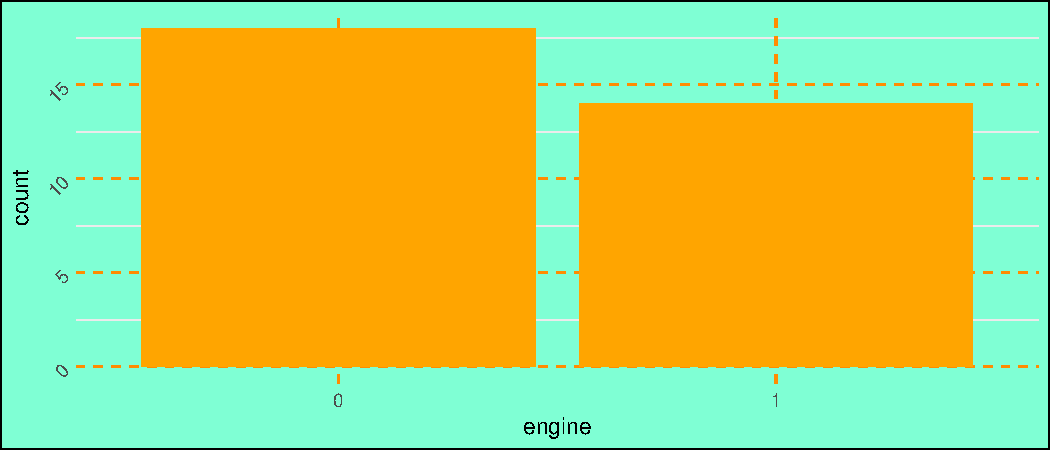
\includegraphics{data-visualization_files/figure-pdf/fig-frequency-and-proportion-of-engine-being-v-shape-or-straight-1.pdf}

}

\end{figure}%

\subsection{Basic Plots}\label{basic-plots}

Plots 1-3 require only data, aesthetics, and geoms. Depending on how you
prepared your data above, you may also need to do very simple
(\textasciitilde1 line) transformation on \texttt{mtcars.viz} before
piping into the \texttt{ggplot()} function.

\subsubsection{Histogram}\label{histogram}

Recreate this histogram of car weight:

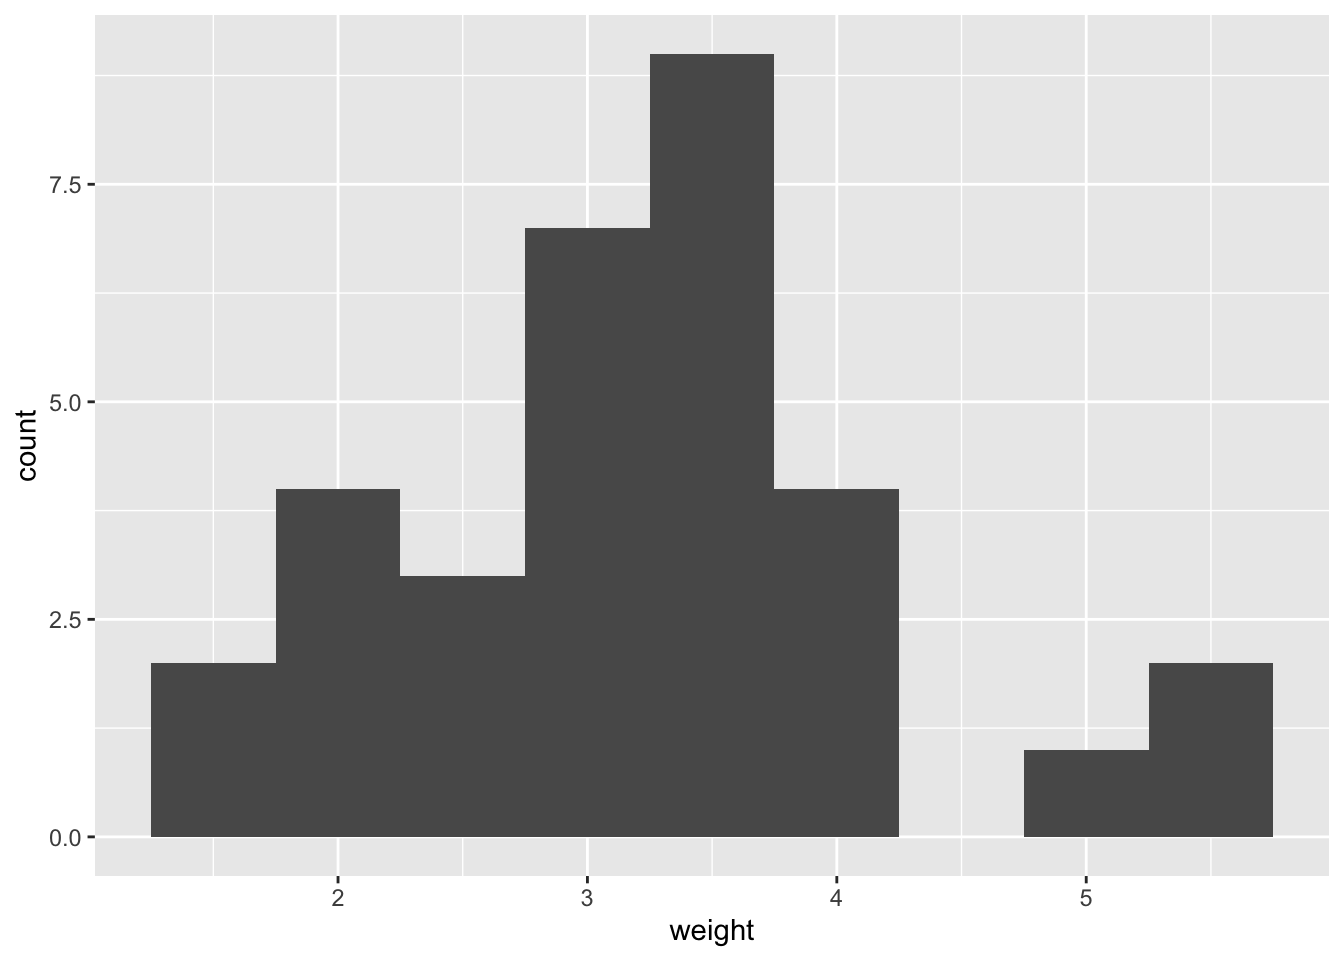
\includegraphics{plots/plot1.png} Figure~\ref{fig-plot1-histogram} shows
my attempt to graph out the histogram graph.

\begin{figure}[!htbp]

{\caption{{Counting by weight}{\label{fig-plot1-histogram}}}}

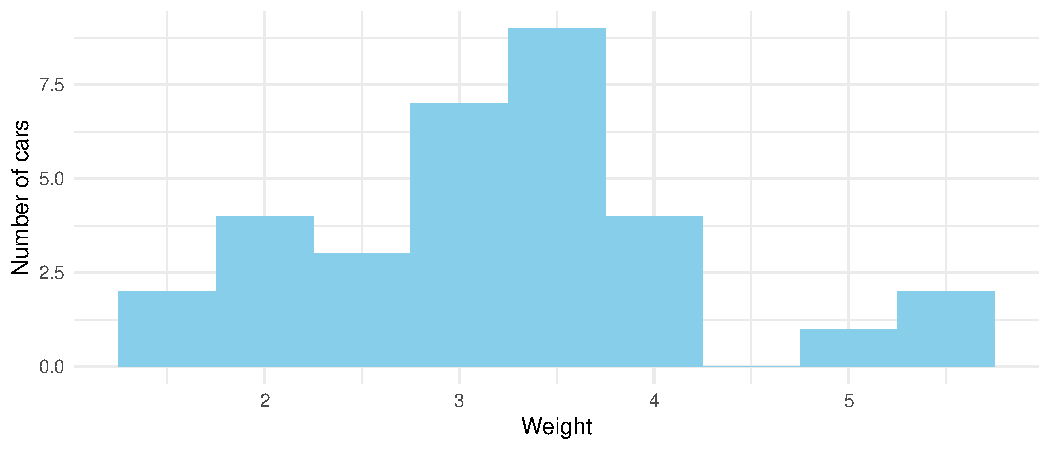
\includegraphics{data-visualization_files/figure-pdf/fig-plot1-histogram-1.pdf}

{\noindent \emph{Note.} The number of cars by weight.}

\end{figure}

\subsubsection{Bar plot}\label{bar-plot}

Recreate this bar plot of the number of cylinders:

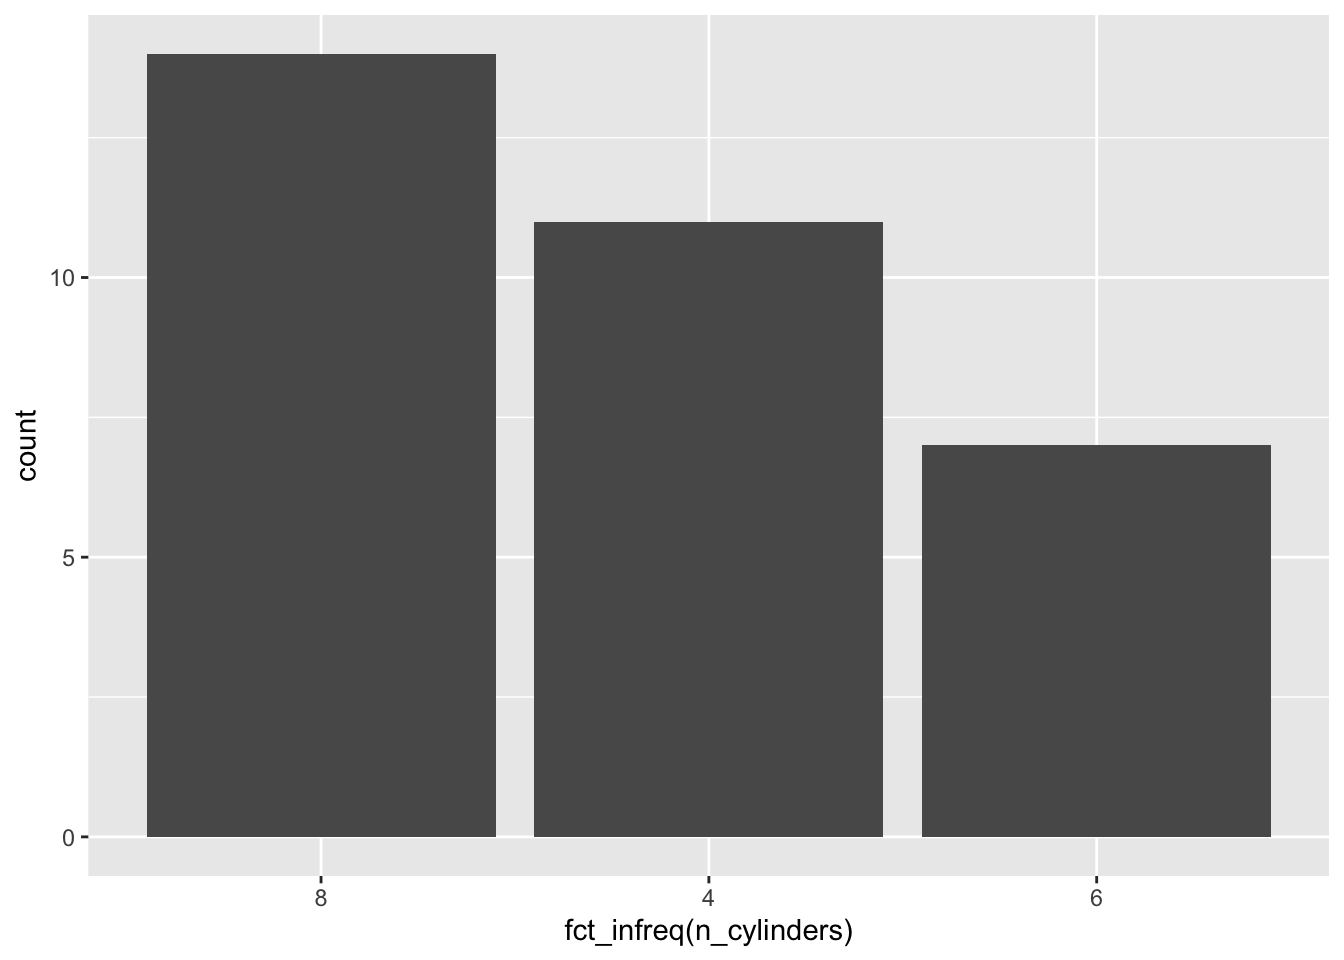
\includegraphics{plots/plot2.png} Figure~\ref{fig-plot2-barplot} shows
my attempt to graph out the barplot.

\begin{figure}[!htbp]

{\caption{{The number of cars by cylinder}{\label{fig-plot2-barplot}}}}

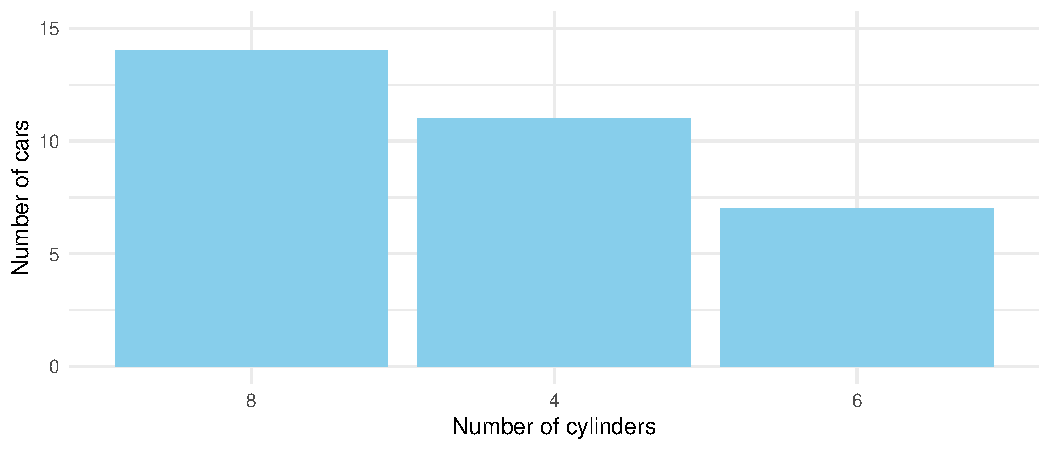
\includegraphics{data-visualization_files/figure-pdf/fig-plot2-barplot-1.pdf}

{\noindent \emph{Note.} This is graph showing the number of cars by
cylinder.}

\end{figure}

\subsubsection{Scatter plot}\label{scatter-plot}

Recreate this scatter plot of car weight vs.~miles per gallon:

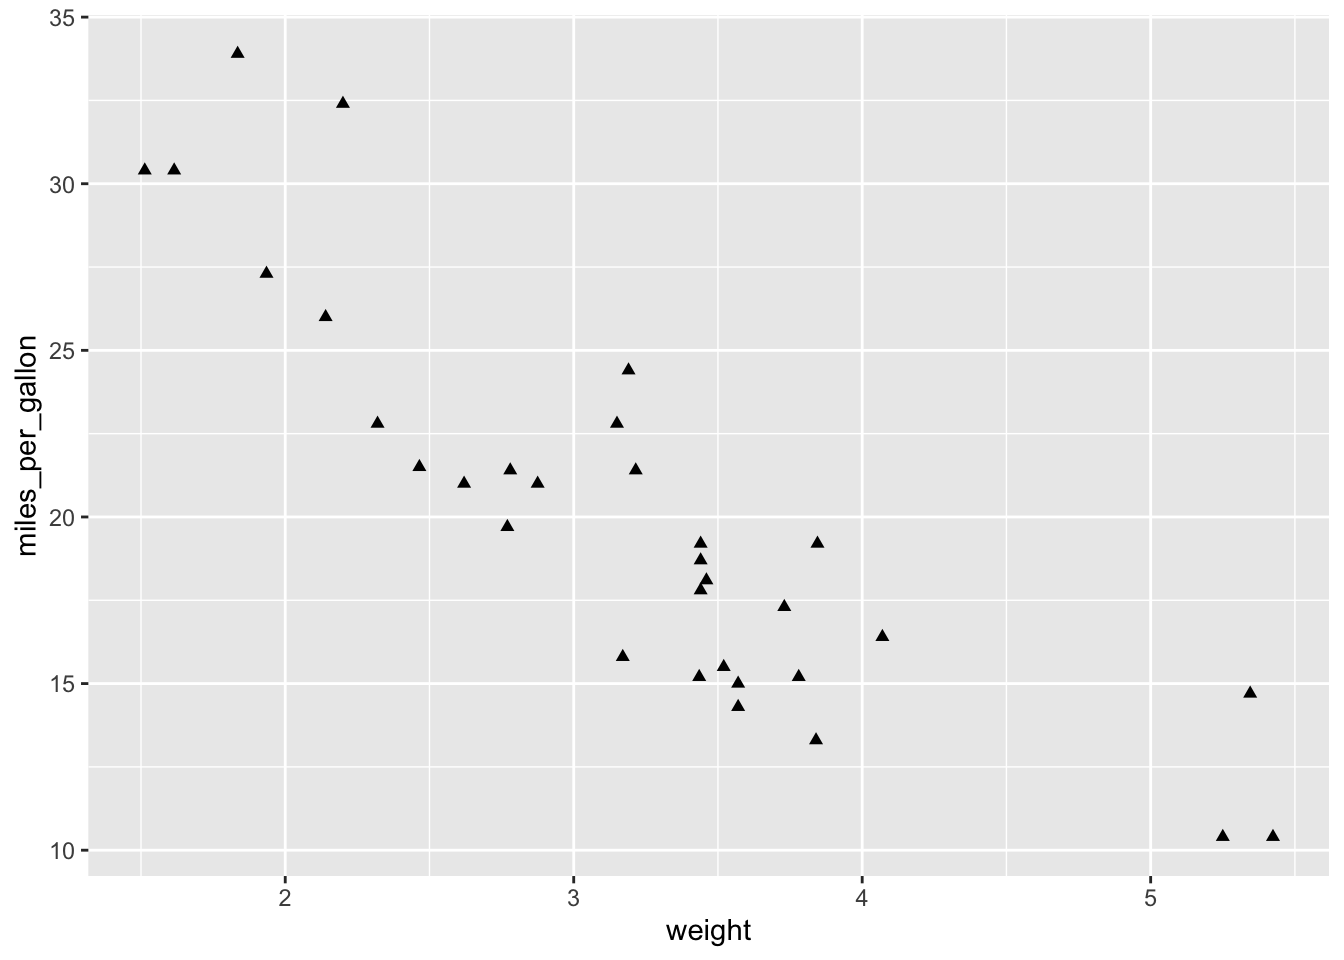
\includegraphics{plots/plot3.png} Figure~\ref{fig-plot3-scatterplot}
shows my attempt to graph out the scatterplot.

\begin{figure}

\caption{\label{fig-plot3-scatterplot}Miles per gallon by car weight}

\centering{

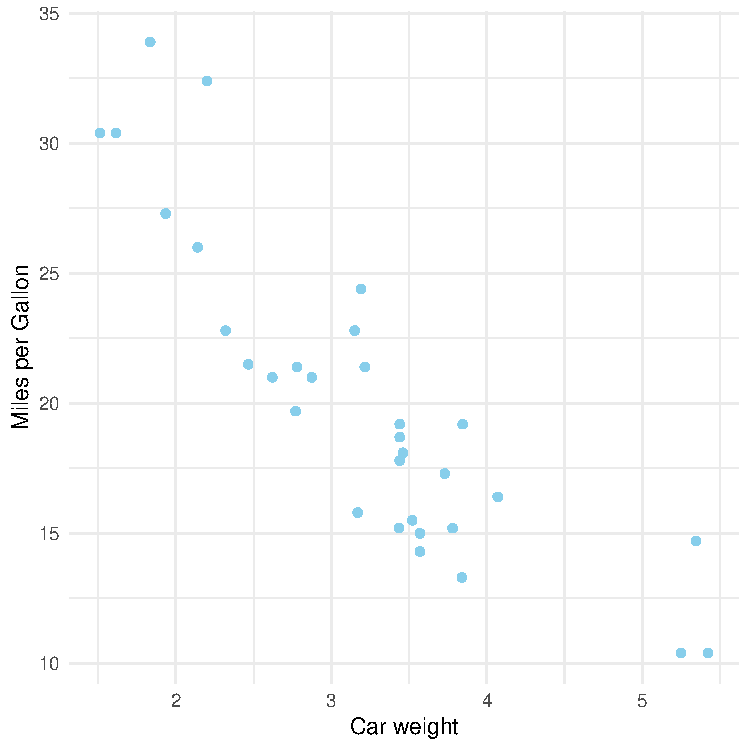
\includegraphics{data-visualization_files/figure-pdf/fig-plot3-scatterplot-1.pdf}

}

\end{figure}%

\subsection{Intermediate Plots}\label{intermediate-plots}

The following three plots require additional layers or aesthetics beyond
the basic plots above, and may require some additional simple data
transformation.

\subsubsection{Box plot}\label{box-plot}

Recreate this box plot of miles per gallon by number of cylinders, with
points showing the distribution:

\begin{figure}[H]

\caption{Box plot of miles per gallon by number of cylinders}

{\centering 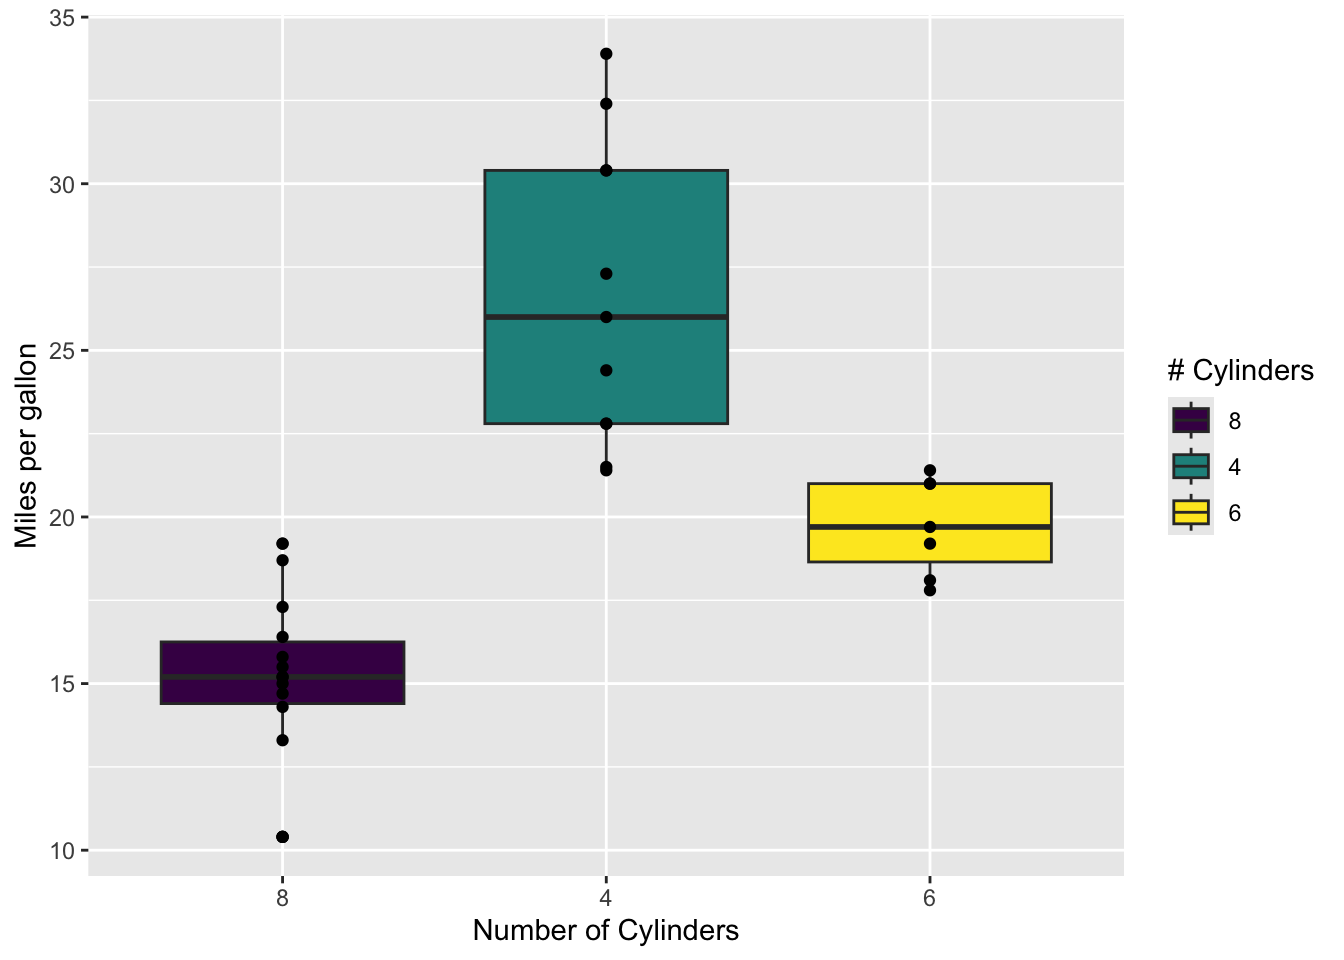
\includegraphics{plots/plot4.png}

}

\end{figure}%

What transformation, if any, do you need to make to the data before
piping it into \texttt{ggplot()}?

turn cylinder into a factor variable and reorder the cylinder into 8, 4,
6.

What geoms and aesthetics are used in this plot? Does layer order
matter, and if so, how?

data points should lie above the scatterplot, so first geom\_boxplot and
then datapoints

What additional information is required to produce this plot? What
layers or aesthetics would you need to add to the plot to include this
information?

the mean for each cylinder type \& the standard deviation.

Figure~\ref{fig-plot4-boxplot} shows my attempt to graph out the
boxplot.

\begin{figure}[!htbp]

{\caption{{Miles per Gallon by cylinder}{\label{fig-plot4-boxplot}}}}

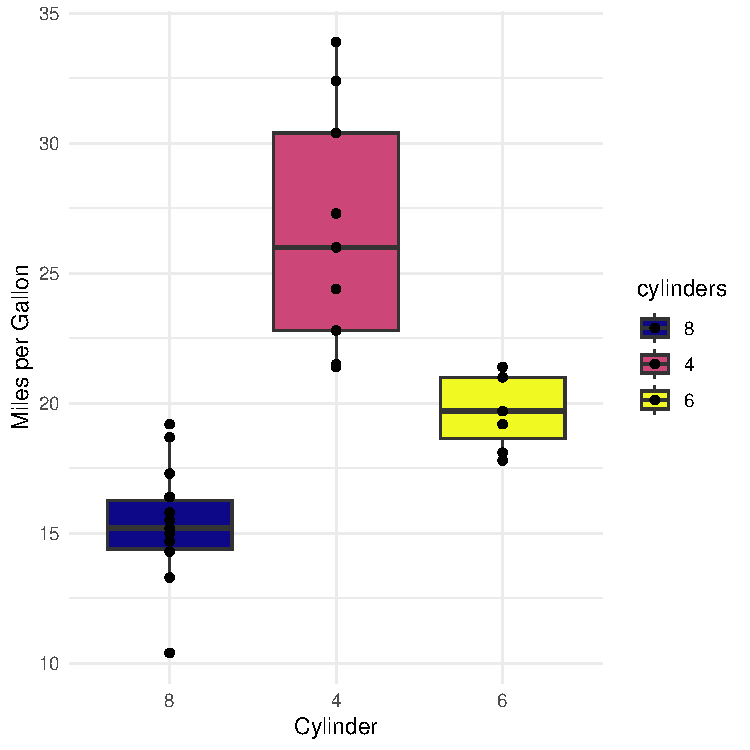
\includegraphics{data-visualization_files/figure-pdf/fig-plot4-boxplot-1.pdf}

{\noindent \emph{Note.} This graph shows miles per gallon when the car
has 4, 6, or 8 cylinders.}

\end{figure}

\subsubsection{Faceted scatter plot}\label{faceted-scatter-plot}

Recreate this faceted scatter plot of car weight vs.~displacement, with
regression lines for each facet:

\begin{figure}[H]

\caption{Faceted scatter plot of car weight vs.~displacement}

{\centering 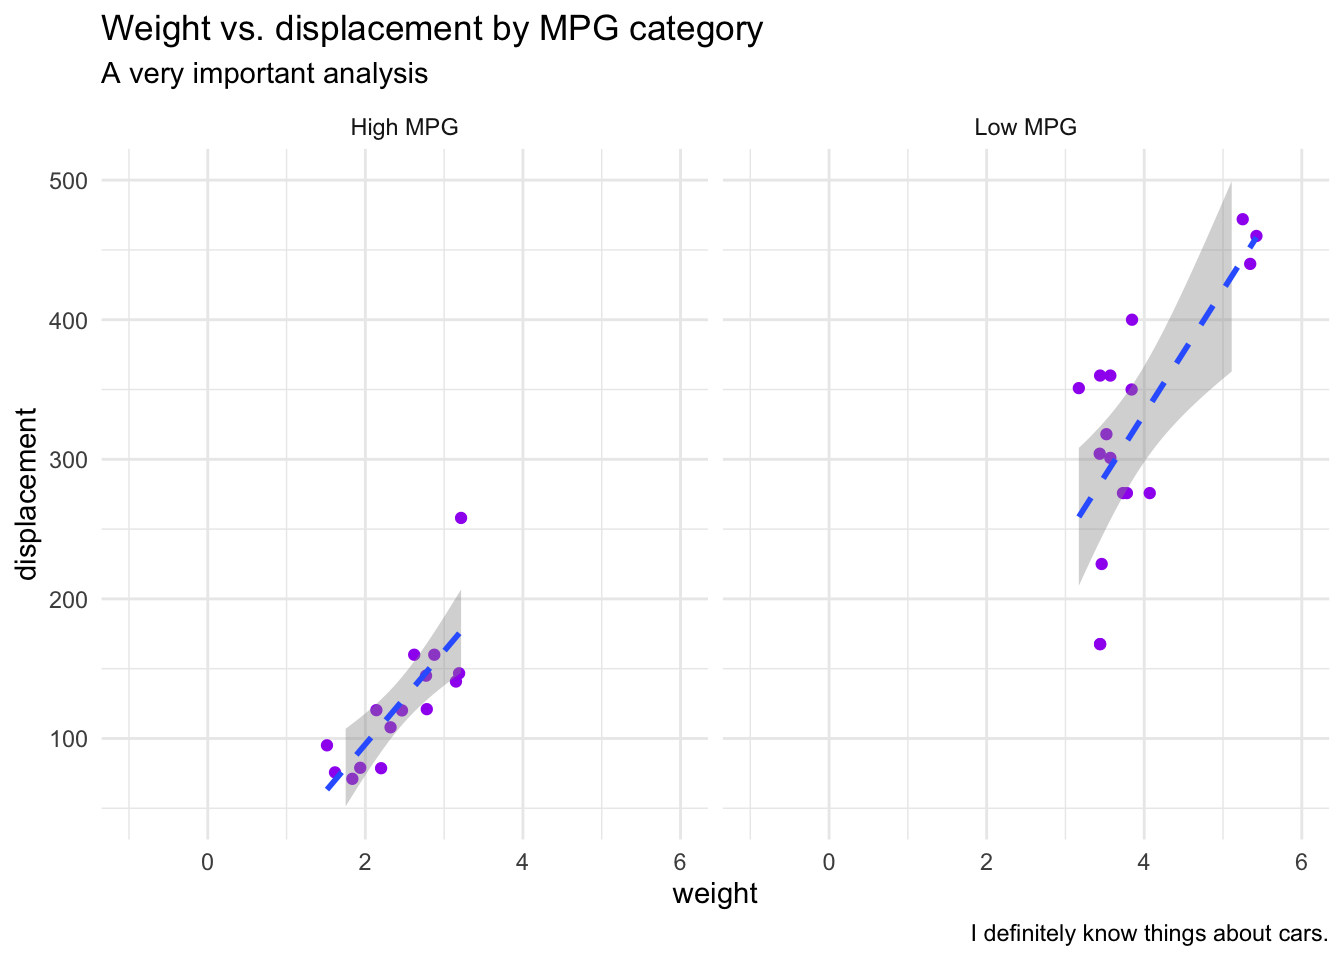
\includegraphics{plots/plot5.png}

}

\end{figure}%

What transformation, if any, do you need to make to the data before
piping it into \texttt{ggplot()}?

MPG has to be separated into low \& high

What geoms and aesthetics are used in this plot? Does layer order
matter, and if so, how?

color fill, line fill, line style.

What additional information is required to produce this plot? What
layers or aesthetics would you need to add to the plot to include this
information?

standard deviation (grey area), slope \& intercept

Figure~\ref{fig-plot5-faceted-scatterplot} shows my attempt to graph out
the faceted scatterplot.

\begin{verbatim}
`geom_smooth()` using formula = 'y ~ x'
\end{verbatim}

\begin{figure}[!htbp]

{\caption{{Weight vs.~displacement by MPG
category}{\label{fig-plot5-faceted-scatterplot}}}}

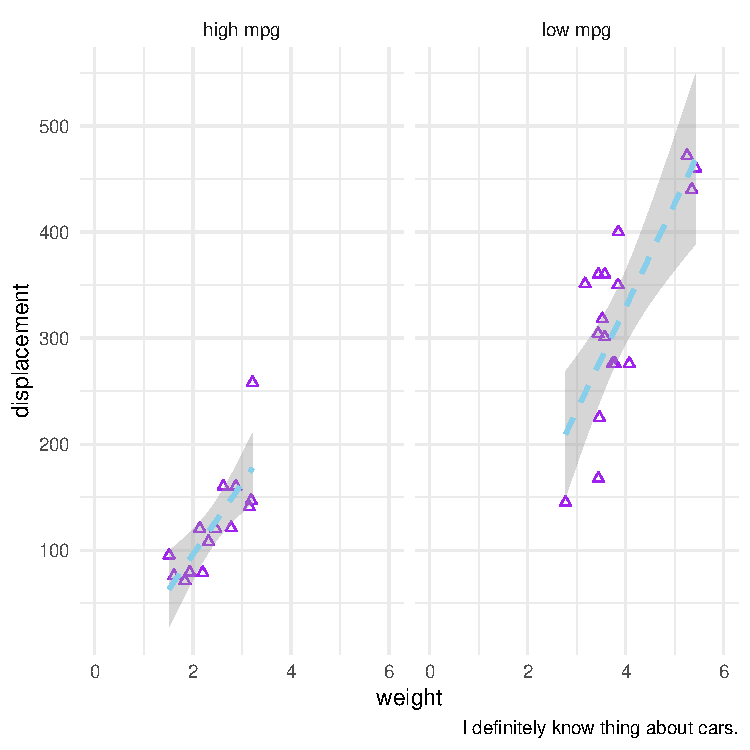
\includegraphics{data-visualization_files/figure-pdf/fig-plot5-faceted-scatterplot-1.pdf}

{\noindent \emph{Note.} Linear regression was used in this example.}

\end{figure}

\subsubsection{Stacked bar plot}\label{stacked-bar-plot}

Recreate this stacked bar plot of transmission type by weight class:

\begin{figure}[H]

\caption{Stacked bar plot of transmission type by weight class}

{\centering 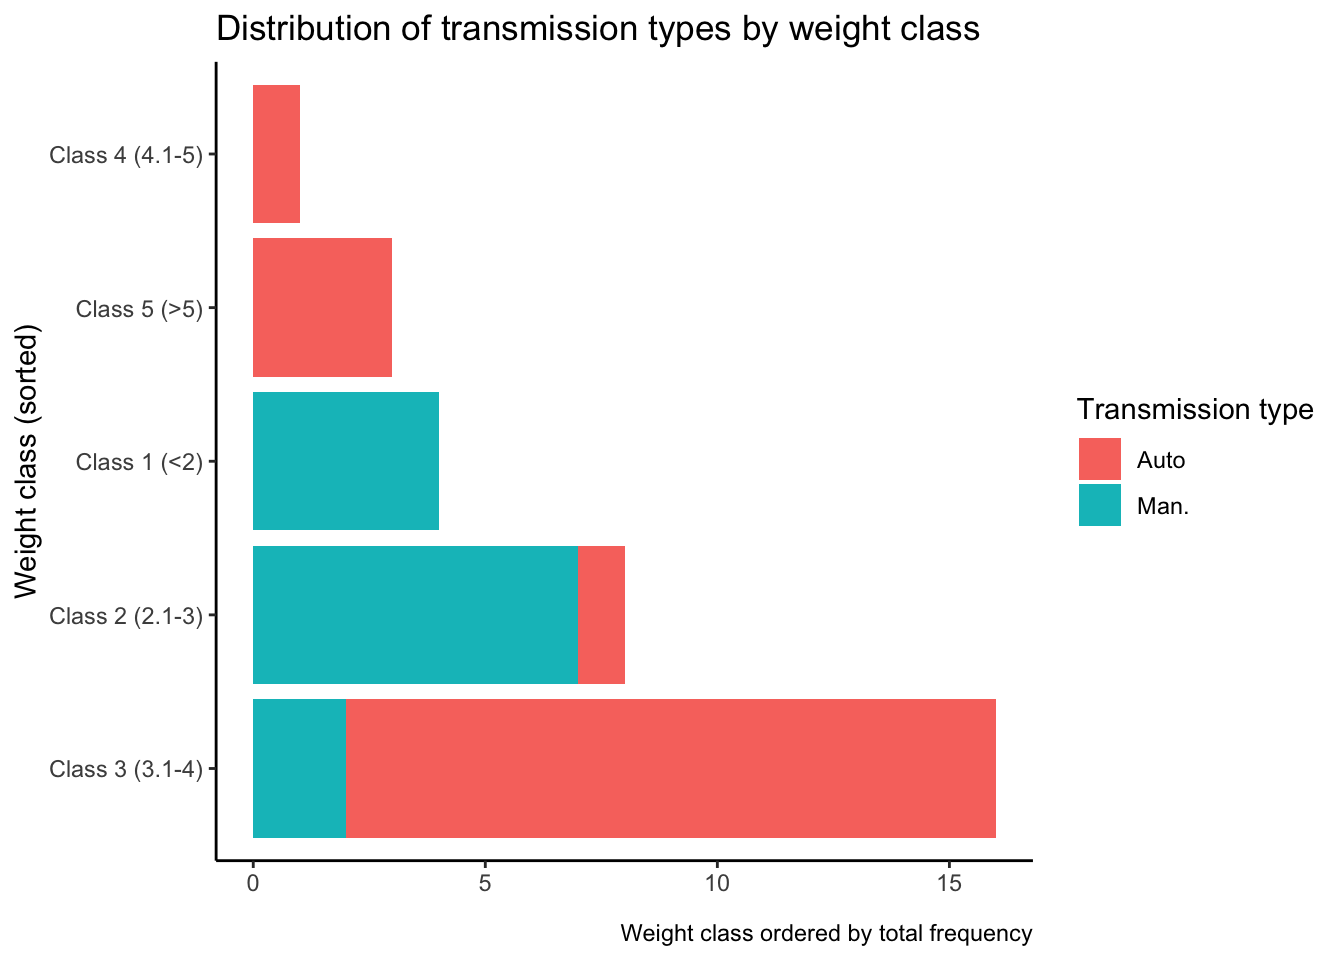
\includegraphics{plots/plot6.png}

}

\end{figure}%

What transformation, if any, do you need to make to the data before
piping it into \texttt{ggplot()}?

We need to categorize weight from class 1-5 \& reorder the classes.
Then, we need to assign auto \& manual to the transmission variable.

What geoms and aesthetics are used in this plot? Does layer order
matter, and if so, how?

Perhaps we can use barplot. The point is to reorder classes by frequency
from lowest and highest.

What additional information is required to produce this plot? What
layers or aesthetics would you need to add to the plot to include this
information?

Figure~\ref{fig-plot6-stacked-barplot} shows my ability to graph out the
stacked barplot.

\begin{verbatim}
# A tibble: 32 x 12
   miles_per_g cylinders displacement horsepower rear_axle_ratio weight
         <dbl>     <dbl>        <dbl>      <dbl>           <dbl>  <dbl>
 1        21           6         160         110            3.9    2.62
 2        21           6         160         110            3.9    2.88
 3        22.8         4         108          93            3.85   2.32
 4        21.4         6         258         110            3.08   3.22
 5        18.7         8         360         175            3.15   3.44
 6        18.1         6         225         105            2.76   3.46
 7        14.3         8         360         245            3.21   3.57
 8        24.4         4         147.         62            3.69   3.19
 9        22.8         4         141.         95            3.92   3.15
10        19.2         6         168.        123            3.92   3.44
# i 22 more rows
# i 6 more variables: mile_time <dbl>, engine <fct>, transmission <fct>,
#   gear <dbl>, carb <dbl>, auto_or_man <chr>
\end{verbatim}

\begin{verbatim}
[1] "Class 2"
\end{verbatim}

\begin{verbatim}
[1] "Class 4"
\end{verbatim}

\begin{figure}

\caption{\label{fig-plot6-stacked-barplot}Stacked barplot of frequency
by weight class categorized by automatic or manual transmission type}

\centering{

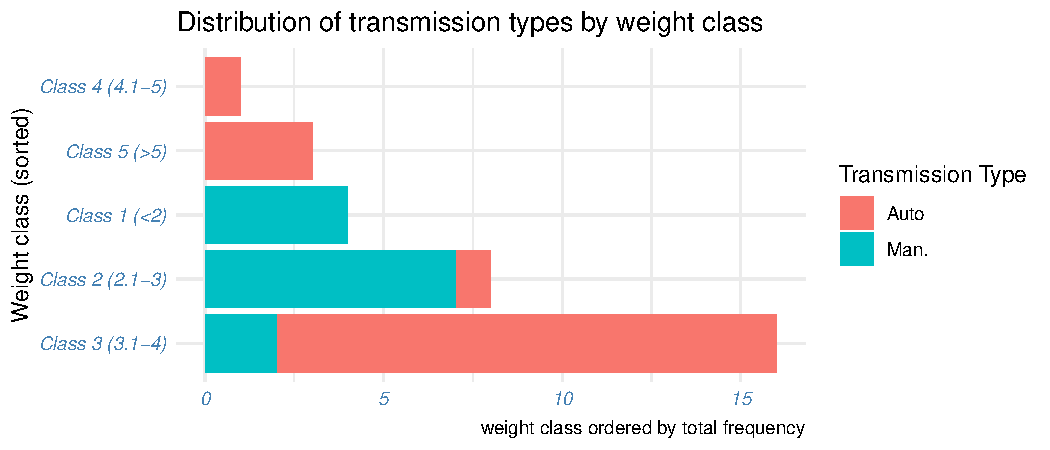
\includegraphics{data-visualization_files/figure-pdf/fig-plot6-stacked-barplot-1.pdf}

}

\end{figure}%

I am testing the function knitr:include\_graphics() that inserts
external image in the folder ``plots'', so I am importing plot 6 from
the folder to compare it with Figure~\ref{fig-plot6-stacked-barplot}.

\begin{figure}

\caption{\label{fig-plot6-for-comparison}}

\centering{

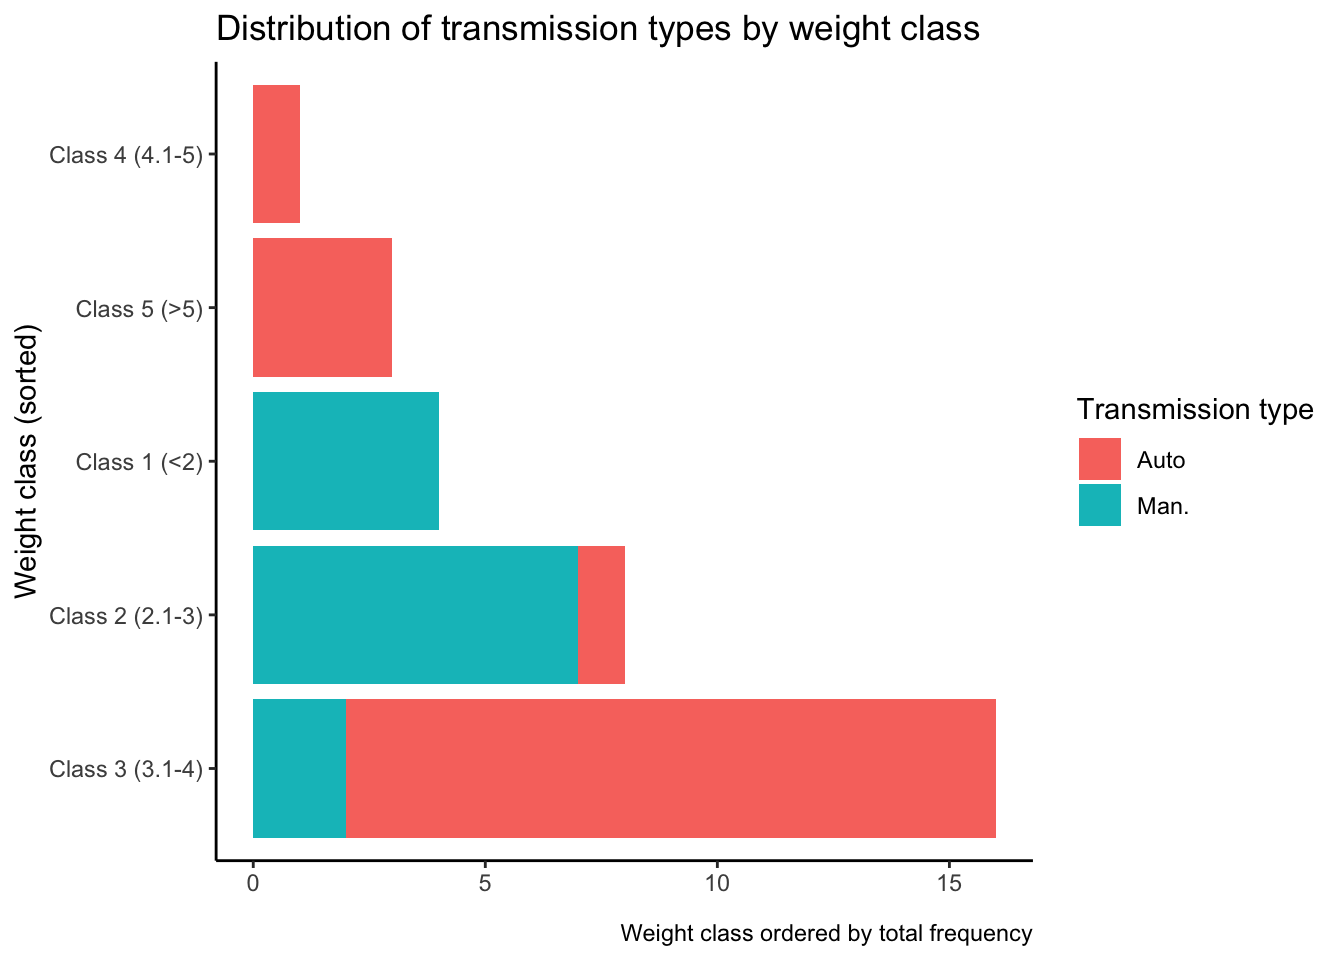
\includegraphics{plots/plot6.png}

}

\end{figure}%

\section{Review}\label{review}

\begin{enumerate}
\def\labelenumi{\arabic{enumi}.}
\tightlist
\item
  Which plots were you able to fully recreate successfully? Did you
  encounter any challenges along the way?
\end{enumerate}

I created all of them. 2. Which plots were you only partially able to
recreate? What challenges did you encounter that limited your ability to
fully recreate the plot? What additional information or skills would you
need to complete the plot?

I need to know what color scheme was used in the original plot 4.

\section{Optional plotting}\label{optional-plotting}

If you have time and would like to practice more, try creating one or
more plots of own design using the \texttt{mtcars.viz} dataset or adding
to one of the plots above. You can use any combination of geoms,
aesthetics, and layers you like. Whether you start from scratch or build
on an existing plot, create your plots in code chunks below. (Leave the
chunks above as your work recreating the plots as-is.)

For each optional plot you create or extend, include a brief description
of the plot below the chunk and any additional information you think is
relevant.

Figure~\ref{fig-optional-plot-1} graphs out the The relationship between
mpg and weight by engine. This graph shows how engine type may lead to
different predictions of mpg on car weight.

\begin{verbatim}
`geom_smooth()` using formula = 'y ~ x'
\end{verbatim}

\begin{figure}

\caption{\label{fig-optional-plot-1}The relationship between mpg and
weight by engine}

\centering{

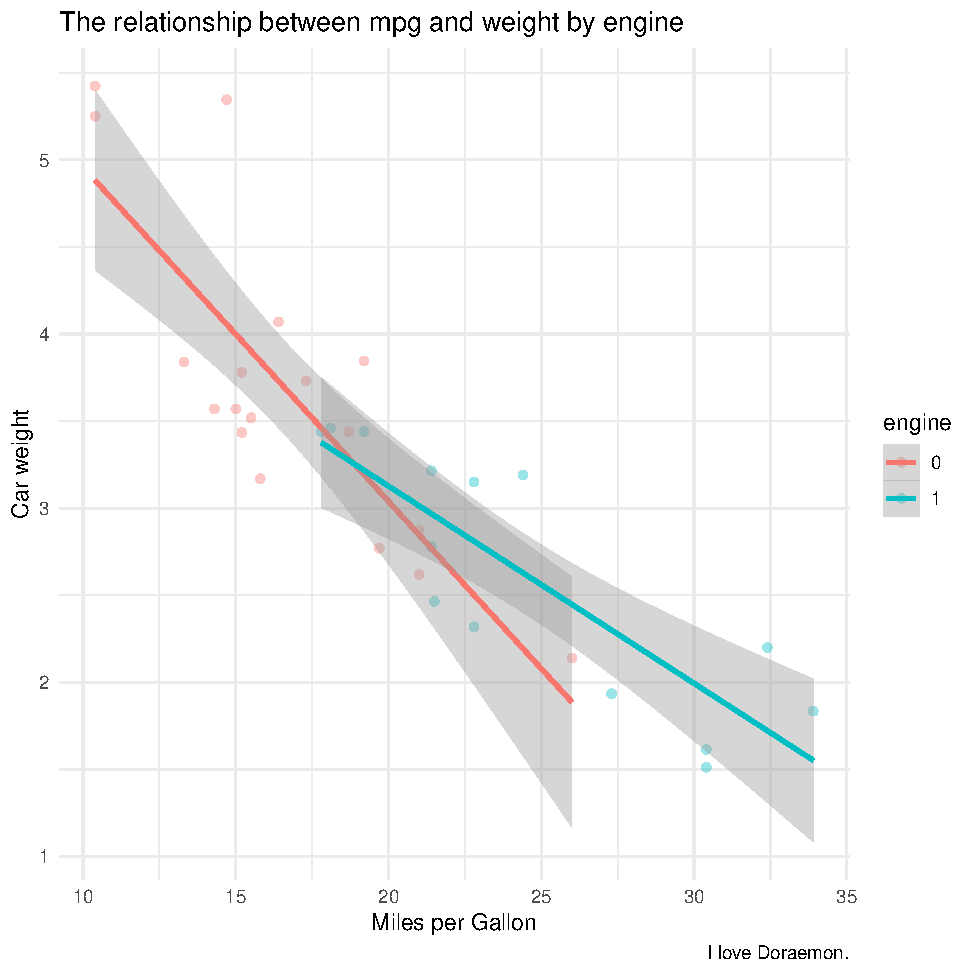
\includegraphics{data-visualization_files/figure-pdf/fig-optional-plot-1-1.pdf}

}

\end{figure}%

\begin{verbatim}
`geom_smooth()` using formula = 'y ~ x'
\end{verbatim}

\section{Submission \& Assessment}\label{submission-assessment}

To submit:

\begin{enumerate}
\def\labelenumi{\arabic{enumi}.}
\tightlist
\item
  Add \& modify the \texttt{assessment.md} in this mini-project's
  directory:

  \begin{enumerate}
  \def\labelenumii{\arabic{enumii}.}
  \tightlist
  \item
    Check off all objectives you believe you have demonstrated
  \item
    Indicate which objectives you are meeting for the first time (if
    any)
  \item
    Complete any relevant open-ended items
  \end{enumerate}
\item
  Push your changes to your centralized assignment repository on GitHub.
\item
  Confirm that Dr.~Dowling and your section TA are added as
  collaborators to your repository.
\item
  Submit your work in your next open mini-project assignment by
  including the following information in the text box:

  \begin{enumerate}
  \def\labelenumii{\arabic{enumii}.}
  \tightlist
  \item
    The title of the assignment: ``Level 1 Data Visualization: Plot the
    mtcars Dataset''
  \item
    A link to the \textbf{directory} for this assignment in your
    centralized assignment repo
  \end{enumerate}
\end{enumerate}






\end{document}
